\section{CAN Bus}

\subsection{Was ist CAN?}
	
Das Controller Area Network ist ein serielles Bus System und wurde
1983, zur Vernetzung von Steuergeräten in Automobilen, von der Firma
Bosch GmbH entwickelt. Doch nicht nur in der Automobilindustrie,
sondern auch in der Medizintechnick, Flug- und Raumfahrttechnik sowie
in Aufzuganlagen und im Schiffsbau, kann man auf einen CAN Bus stoßen
\citep[nach][]{WI1}. Der Vorteil gegüber der herkömmlichen Verkablung
lag darin, das mehrere Knoten über dieselbe Leitung Kommunizieren
können. Alle Teilnehmer können Pakete priorisiert mit
Kollisionserkennung auf den Bus legen, hierbei wird die Nachricht,
nicht der Empfänger adressiert.
\\
Die physikalischen Eigenschaften und der Formale Aufbau des CAN Busses
wird in folgenden ISO Normen genau spezifiziert \citep[nach][]{WI1}:

\begin{itemize}
\item ISO 11898-1:2003 Road vehicles — Controller area network — 
Part 1: Data link layer and physical signalling
\item ISO 11898-2:2003 Road vehicles — Controller area network — 
Part 2: High-speed medium access unit
\item ISO 11898-3:2006 Road vehicles — Controller area network — 
Part 3: Low-speed, fault-tolerant, medium dependent interface
\item ISO 11898-4:2004 Road vehicles — Controller area network — 
Part 4: Time-triggered communication
\item ISO 11898-5:2007 Road vehicles — Controller area network — 
Part 5: High-speed medium access unit with low-power mode
\item ISO/NP 11898-6 Road vehicles — Controller area network — 
Part 6: High-speed medium access unit with selective wake-up functionality
\end{itemize}

\subsubsection{Übertragungsgeschwindigkeiten}

Aufgrund der Ausbreitungsgeschwindigkeit der Signale auf dem Bus, ist die 
Übetragungsgeschwindigkeit von der Leitungslänge abhängig. Die Tabelle 
\ref{tab:speed} beinhaltet eine Zuordnung von Leitungslängen und deren 
maximaler Übertragunsgeschwindigkeit und andersrum.

\begin{table}[h]
	\centering
	\begin{tabular}{lcr}
		Bus Speed & Bus Length \\
		\hline
		1 Mbit/s & 40m \\
		500 kbit/s & 100m \\
		125 kbit/s & 500m \\
		50 kbit/s & 1 km \\
	\end{tabular}
	\label{tab:speed}
	\caption{Übertragungsgeschwindigkeiten}
\end{table}

\subsubsection{Einsatzgebiete}

CAN-Protokolle haben sich in verschiedenen, vor allem sicherheitsrelevanten 
Bereichen etabliert, bei denen es auf hohe Datensicherheit ankommt 
\citep[nach][]{WI1}. Beispiele:

\begin{itemize}
\item Automobilindustrie (Vernetzung unterschiedlicher Steuergeräte, Sensoreinheiten 
und sogar Multimediaeinheiten)
\item Automatisierungstechnik (zeitkritische Sensoren im Feld, Überwachungstechnische 
Einrichtungen)
\item Aufzugsanlagen (Vernetzung der Steuerung mit verschiedenen Sensoren, Aktoren 
und Aufzugsanlagen untereinander innerhalb einer Aufzugsgruppe)
\item Medizintechnik (Magnetresonanz- und Computertomographen, Blutgewinnungsmaschinen,
 Laborgeräte, Elektro-Rollstühle, Herzlungen-Maschinen)
\item Flugzeugtechnik (Vernetzung innerhalb von Kabinen- und Flugführungssystemen)
\item Raumfahrttechnik (vermehrte Verwendung in parallelen Busarchitekturen)
\item Beschallungsanlage (wird für die Steuerung von digitalen Endstufen verwendet)
\item Schienenfahrzeuge
\item Schiffbau (Die DGzRS lässt in die neue Generation ihrer Seenotrettungskreuzer 
Bus-Systeme einbauen.)
\end{itemize}

\subsection{Busankoplung}

Der CAN Bus arbeitet nach dem Multi-Master Prinzip, wonach es jedem Knoten 
möglich ist, mit jedem anderen Knoten zu kommunizieren. Üblicherweise in 
Linientopologie aufgebaut, können laut ISO 119898 bis zu 32 Knoten damit
verbunden werden. Die Signalübetragung erfolgt symmetrisch.

Für die physische Verbindung zwischen den einzelnen CAN-Knoten werden in der Praxis
häufig Unshielded Twisted Pair Leitungen verwendet. An den Enden des CAN-Netzwerks 
sorgen Busabschlusswiderstände für die Vermeidung von Ausgleichsvorgängen (Reflexionen).

\begin{figure}[h] 
\centering
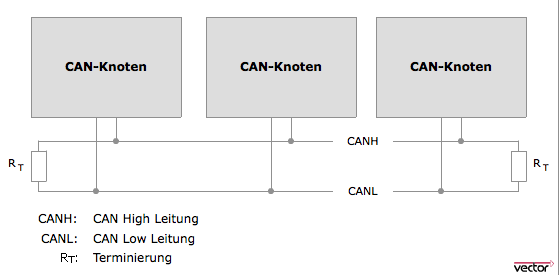
\includegraphics[width=0.9\textwidth]{figures/cannet}
\caption{Vernetzung von CAN Knoten \citep{VEC}} 
\label{pic:cannet}
\end{figure}

\subsection{CAN-Bus Pegel} 

Auf dem physischen Medium werden die einzelnen Bits über Spannungsdifferenzen
abgebildet. Man unterscheidet hier zwischen Highspeed-CAN (Abb. \ref{pic:highcan}) 
und Lowspeed-CAN (Abb. \ref{pic:lowcan}).

Für die reibungslose Kommunikation, vor allem für den Buszugriff, die Fehlersignalisierung 
und für das Acknowledgement, unterscheidet man zwischen einem dominanten und einem 
rezessiven Buspegel. Der dominante Buspegel entspricht der logischen ``0''. Der rezessive 
Buspegel entspricht der logischen ``1''. 

Wenn versciedene Teilnehmer gleichzeitig einen dominanten und einen rezessiven Pegel senden, 
so überschreibt immer der dominante Pegel den rezessiven Pegel auf dem CAN-Bus (siehe 
Kapitel \ref{sec:access}). Der rezessive Buspegel stellt sich nur dann ein, wenn alle CAN-Knoten 
rezessiv senden. 

\begin{figure}[h] 
\centering
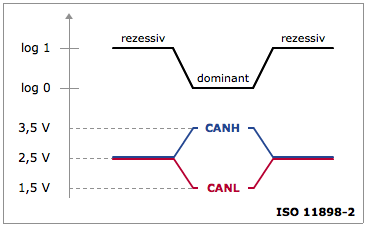
\includegraphics[width=0.7\textwidth]{figures/highcan}
\caption{Highspeed-CAN Buspegel \citep{VEC}} 
\label{pic:highcan}
\end{figure} 

\begin{figure}[h] 
\centering
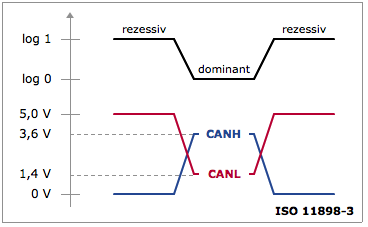
\includegraphics[width=0.7\textwidth]{figures/lowcan}
\caption{Loewspeed-CAN Buspegel \citep{VEC}} 
\label{pic:lowcan}
\end{figure}

\clearpage
\newpage
\subsection{Bit Stuffing}
\label{sec:bitstuffing} 
Bit-Stuffing beim CAN-Bus bedeutet, dass
nach 5 Bits mit gleichem Pegel ein ">Stuff Bit"< mit inversem Pegel
eingefügt wird. Die Empfänger filtern diese Stuff-Bits, dann nach dem
gleichen Schema wieder heraus.
\\ Bit stuffing wird einerseits
eingesetzt, weil Bitfolgen mit mehr als 5 Bits mit gleichem Pegel für
Steuerungszwecke eingesetzt werden, und andererseits auch wegen der
NRZ-Kodierung. Das heißt dass der Pegel bei zB 4 rezessiven Bits
gleich bleibt. Wenn dann beispielsweise 10 gleiche Bits übertragen
werden, so kann der Empfänger möglicherweise nicht mehr unterscheiden,
ob jetzt 10 oder 11 Bits übertragen wurden.
	
\subsection{CAN Frames} Beim CAN-Bus gibt es 4 unterschiedliche Arten
von Frames: 
\begin{itemize} 
\item Daten-Frame 
\item Remote-Frame 
\item Error-Frame 
\item Overload-Frame 
\end{itemize} 

\subsubsection{Daten Frame} 
Die Daten-Frames dienen dem Transport von Daten und können bis
zu 8 Byte an Nutzdaten enthalten. Bei den Daten-Frames kann zwischen
Standard Format und Extended Format unterschieden werden, die sich
hauptsächlich in der Länge des Identifiers unterscheiden. Der Aufbau
eines Daten Frames kann aus Abbildung \ref{data} entnommen werden.
	
\begin{figure}[h] 
\centering
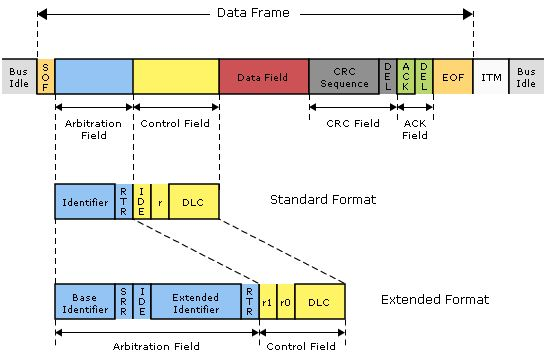
\includegraphics[width=0.9\textwidth]{figures/data-frame}
\caption{Aufbau eines Daten-Frames \citep{HYC}} 
\label{data}
\end{figure} 
%Quelle: http://marco.guardigli.it/2010/10/hacking-your-car.html
		
Gestarted wird ein Frame durch das \textbf{SOF} (start-of-frame)
bestehend aus einem dominanten Bit, das der Synchronisation aller CAN-Knoten dient. Darauf folgt gleich das
Arbitrationsfeld und dem Kontrollfeld. Abhängig vom Format bestehen
diese aus \textbf{Basis Identifier} (11 Bits), \textbf{Extended
Identifier} (18 Bit), einem \textbf{RTR}-Bit (remote transmission
request; bei Remote-Frames rezessiv) sowie einem \textbf{SRR}-Bit
(substitude-remote-request; rezessiv). Ist das \textbf{IDE}-Bit
(identifier extension) rezessiv, so handelt es sich um das Extended
Format, das somit immer Nachrang über dem Standard Format hat.\\ Im
Kontrollfeld befindet sich neben 1-2 reservierten (aktuell nicht
verwendeten) Bits der aus 4 Bits bestehende \textbf{DLC} (data length
code), der die Länge des nachfolgenden \textbf{Datenfeldes} angibt.\\
Wie bereits erwähnt können mit den Daten-Frames bis zu 8 Byte, also 64
Bit, übertragen werden. dies kann jedoch nur in einheiten von 8 Bits
geschehen. Anschließend an das Datenfeld ist das CRC-Feld (cyclic
redundancy check; Prüfsummenfeld) bestehend aus 16 Bit (15 Bit + 1
rezessives Delimiter-Bit). Des weiteren enthält ein Daten-Frame ein
\textbf{ACK}-Feld (Acknowledge). Dieses wird verwendet, um den Empfang
eines korrekten Frames zu bestätigen. Der Sender sendet dafür ein
rezessives Bit. Jeder Empfänger der keinen Fehler feststellen konnte,
setzt einen dominanten Pegel und überschreibt somit den rezessiven des
Senders. Im Falle einer negativen Quittierung (rezessiver Pegel) muss
der Knoten, der den Fehler erkannt hat, nach dem ACK-Delimiter einen
Error-Frame aussenden.\\Das Ende des Frames wird mit 7 rezessiven Bits
dem \textbf{EOF} (end of frame) angezeigt. Anschließend an den Frame
muss ein ITM-Package (intermission oder inter-frame-space) bestehend
aus mindestens 3 rezessiven Bits gesendet werden.
	
\subsubsection{Remote Frame} Mit Hilfe der Remote-Frames können
Daten-Frames von anderen Teilnehmern angefordert werden. Der Frame
unterscheidet sich vom Daten-Frame durch ein rezessives Bit im
">RTR"<-Slot, wodurch Remote-Frames im Falle einer Kollision immer
Nachrang gegenüber den Daten-Frames haben, und durch ein Fehlen des
Datenfeldes.
	
\subsubsection{Error Frame} Erkennt ein CAN-Knoten einen Fehler, so
sendet er einen Error-Frame an alle anderen CAN-Knoten im Netzwerk.
Bei diesen Frames wird das Bit-Stuffing bewusst ignoriert. Der
Error-Frame besteht aus 2 Feldern, den Error-Flags und dem
Error-Delimiter (8 rezessive Bits). Die Error-Flags sind abhängig vom
Modus in dem sich ein CAN-knoten befindet. Ist der Knoten im
Fehler-Status \textit{">error active"<} so setzt er die Error-Flags
auf 6 dominante Bits. Befindet er sich hingegen im Fehler-Status
\textit{">error passive"<} so sendet er 6 rezessive Bits.
	
\subsubsection{Overload Frame} Overload-Frames werden als Zwangspause
zwischen Daten- und Remote-Frames genutzt. Dabei hat ein
Overload-Frame das gleiche Format wie ein Active-Error-Frame. Wie in
Abbildung \ref{overload} ersichtlich ist, besteht der Overload-Frame
ebenfalls aus 2 Feldern: dem Overload-Flag (6 dominante Bits) und dem
Overload-Delimiter (8 rezessive Bits). Ein Overload-Frame kann jedoch
nur während eines Interframespaces gesendet werden. Dies ermöglicht
die Unterscheidung von den Error-Frames, die während der Übertragung
einer Nachricht gesendet werden, sobald eben ein Fehler erkannt wurde.

	
\begin{figure}[h] 
\centering
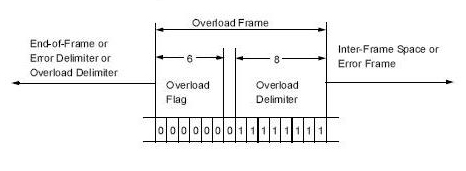
\includegraphics[width=0.7\textwidth]{figures/overload-frame}
\caption{Aufbau eines Overload-Frames \citep{CBM}} 
\label{overload}
\end{figure} 
% Quelle: http://rs232-rs485.blogspot.co.at/2009/11/can-bus-message-frames-overload.html
	
\subsection{Zeichenkodierung}
	
Auf der Busleitung werden die einzelnen Bits der Pakete über den 
Non-Return-to-Zero Code (NRZ) codiert. Hierbei hat jeder Wert eines Bit 
einen konstanten Zusatand auf der Leitung (siehe Abb. \ref{nrzcode}).

\begin{figure}[h] 
\centering
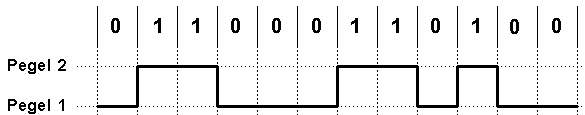
\includegraphics[width=0.9\textwidth]{figures/nrzcode}
\caption{NRZ-Code \citep{NRZ}} 
\label{nrzcode}
\end{figure} 

Probleme bei dieser Codierung können auftreten, wenn mehrere gleiche Symbole in Folge
gesendet werden. Abhilfe schafft hier Bit-Struffing, näheres dazu in Kapitel ~\ref{sec:security}.

Als Vergleich zur NRZ Codierung sollte man noch den Manchester-Code erwähnen, bei dem
jeweils eine steigende, bzw. fallende Taktflanke einen Bit-Wert repräsentiert (Abb. \ref{mancode}).
Ein Bitstuffing ist hier nicht nötig, da auch gleiche aufeinanderfolgende Bits durch eine Taktflanke 
reproduzierbar sind.

\begin{figure}[h] 
\centering
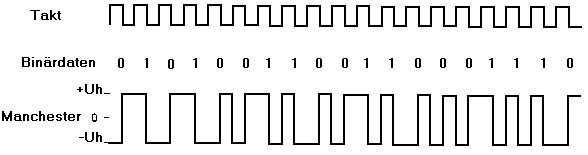
\includegraphics[width=0.9\textwidth]{figures/mancode}
\caption{Manchester-Code \citep{MAN}} 
\label{mancode}
\end{figure} 
	
\subsection{Synchronisatzion}

Da die CAN Knoten nur eine gemeinsame Baud-Rate, jedoch keinen gemeinsamen Takt besitzen, 
wird der Daten-Frame selbst zur Synchronization verwendet. Es gibt eine Hard- und eine Soft-Synchronization,
wobei die Hard-Synchronization die fallende Flanke des Startbits zur Synchronizierung verwendet. Alle 
nachfolgenden abfallenden Flanken werden zur Soft-Synchronizierung verwendet. Durch die Soft-Synchronizierung
kann sich der Takt nur noch in einem spezifizierten Rahmen verschieben \citep[nach][]{BSY}.
	
\subsection{Buszugriffsverfahren}
\label{sec:access}

Durch die Multi-Master-Architektur des CAN-Bus kann es passieren, dass mehrere Knoten gleichzeitig veruschen
Daten über den Bus zu senden denn jeder Knoten hat das Recht zu jederzeit und ohne Absprache Daten zu senden.
Um dieses Szenario zu vermeiden, bzw. aufzulösen verwendet man CMSA/CA (Carrier Sense Multiple 
Access/Collision Avoidance). Bei diesem Verfahren ``lauscht'' jeder Teilnehmer vor dem Senden ob der Bus frei ist.

Sollte es durch simultanen Zugriff dennoch zu einer Collision kommen, wird durch eine bitweise Arbitrierung.
Über den Basis Identifier im Arbitrationsfeld des Pakets wird dann entschieden, wer den Zugriff auf den Bus bekommt.
Entscheidend ist hier, welche Nachricht die höhere Priorität besitzt, bzw. als erstes ein rezessives Bit sendet.

\begin{figure}[h] 
\centering
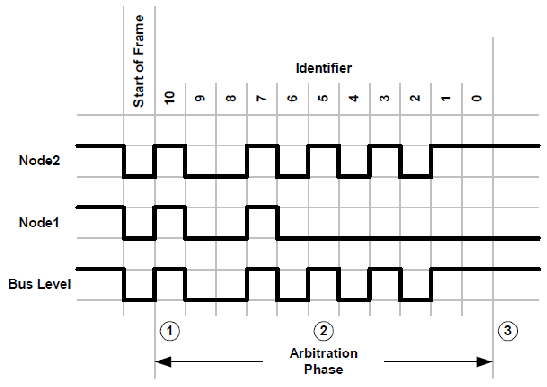
\includegraphics[width=0.9\textwidth]{figures/bitwisearb}
\caption{Beispiel: Bitweise Arbitrierung \citep{BWA}} 
\label{pic:bitwise}
\end{figure} 

Abbildung \ref{pic:bitwise} zeigt ein Beispiel der bitweisen Arbitrieung. An Punkt (1) beginnen beide 
Knoten gleichzeitig mit dem senden Ihres Identifieres. Node 2 sendet an der 5. Bistelle des Identifiers 
ein dominantes Bit, wohingegen Node 1 ein rezessives Bit sendet. An diesem Punkt (2) beendet 
Node 1 seine Übetragung und der Bus gehört Node 2.

Der Identifier addressiert die Nachricht und dient gleichzeitig als Priorisierung. Jeder Identifier kann 
nur einen Sender, jedoch mehrere Empfänger haben.

\subsection{Sicherungsmechanismen und Fehlererkennung}
\label{sec:security}

Für die Fehlererkennung stehen gleich mehrere Verfahren zur Verfügung:

\subsubsection{Bitmonitoring}

Dies ist Aufgabe des Senders. Er vergleicht ob das gesendete Bit mit dem Buspegel übereinstimmt. 
Sollten diese nicht übereinstimmen wird mit die Fehlerbehandung eingeleitet. Auf das Arbitration Field 
und den ACK-Slot findet dieses Verfahren keine Anwendung.

\subsubsection{Stuff Check}

Dies ist Aufgabe des Empfängers. Sollte diese sechs homogene Bits lesen, liegt ein Bitstuffing-Fehler 
vor (siehe Kapitel \ref{sec:bitstuffing}). Auch diese zieht eine Fehlerbehandlung nach sich.

\subsubsection{Form Check}

Auch dies ist Aufgabe des Empfängers. Er vergleicht den ankommenden Bitstrom mit dem Datenformat.
Ein dominantes Delimiter-Bit (CRC oder ACK) oder ein dominantes Bit im EOF signalisiert einen 
Formatfehler und leitet eine Fehlerbehandlung ein.

\subsubsection{Cyclic Redundancy Check}

Der Empfänger überprüft die ankommenden Bits mit der CRC Sequence. Ein Fehler leitet eine 
Fehlerbehandlung ein.

\subsubsection{ACK Check}
	
Sollte das im ACK Slot gesendete rezessive Bit nicht von mindestens einem Empfänger überschrieben 
werden, liegt ein Bestätigungsfehler vor, der eine Fehlerbehandlung nach sich zieht.

Abbildung \ref{pic:errcheck} verdeutlicht das Auftreten der jeweiligen Fehler in den einzelnen Bereichen
einer Nachricht.

\begin{figure}[h] 
\centering
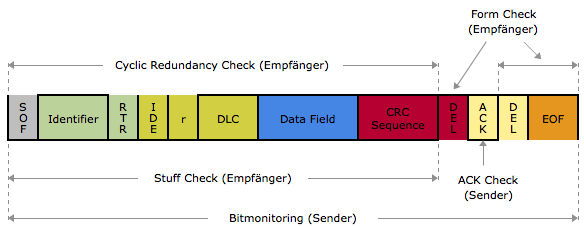
\includegraphics[width=0.9\textwidth]{figures/errcheck}
\caption{Fehlererkennung \citep{VEC}} 
\label{pic:errcheck}
\end{figure} 

\subsubsection{Fehlerbehandlung}

Sollte ein Fehler erkannt werden, sendet der jeweilige CAN-Knoten ein Fehlersignal (Error-Flag). Dieser
besteht aus sechs dominanten Bits, welcher absichtlich die Bitstuffingregel verletzt. Durch den Error-Flag
werden alle Teilnehmer des CAN über einen Fehler informiert (Bitstuffingfehler).

\subsection{Fehlerverfolgung}

Um die Netzweite Datenkonsitenz sicherzustellen, können, wie oben schon erwähnt, alle Knoten die einen 
Fehler erkennen die Nachricht auf dem Bus abbrechen. Hierbei kann es auch vorkommen das dies 
irrtümlicherweise geschieht.

Jeder CAN-Controller besitzt eine Sendefehlerzähler (TEC, Transmit Error Counter) und einen 
Empfängerfehlerzähler (REC, Receive Error Counter). Nach jeder erfolgreichen Übertragung eines 
Data oder Remote Frames veringert sich der jeweilige Fehlerzähler (TEC=TEC-1; REC=REC-1). 
Enteckt ein Knoten einen Fehler und sendet einen Error Flag wird der entsprechende Fehlerzähler 
erhöht. Hierbei gilt für den Sender: TEC=TEC+8 für den fehlererkennenden Empfänger: REC=REC+1.
Für den Fehler verursachenden Empfänger gilt zudem REC=REC+8.

Je nach höhe des Fehlerzählers gibt es verschidene Zustände des CAN-Knotens. Zu Beginn befinden
sich alle Knoten im ``Active Error''-State. In diesem Modus werden vom CAN-Knoten Error Flags beim 
erkennen eines Fehlers gesendet. Sollte einer der Fehlerzähler (TEC oder REC) über 127 steigen, fällt 
der CAN-Knoten in den ``Error Passive''-State. In deisem Zustand können entdeckte Fehler lediglich 
mit sechs homogenen rezessiven Bits signalisiert werden. Fehlererkennenden Empfängern wird so die 
Möglichkeit genommen, entdeckte Fehler zu globalisieren. Knoten, die sich im „Error Passive“-State 
befinden, müssen beim Senden von zwei aufeinanderfolgenden Data oder Remote Frames zusätzlich 
die „Suspend Transmission Time“ (8 Bits) abwarten.

Sollte der TEC über 255 steigen geht der CAN-Knoten in den ``Bus Off''-State und trennt sich damit
vom Bus ab. Der Zustand Bus Off kann nur durch Eingriff des Host (mit 128 x 11 Bit Zwangswartezeit) 
oder per Hardware-Reset verlassen werden.

\begin{figure}[h] 
\centering
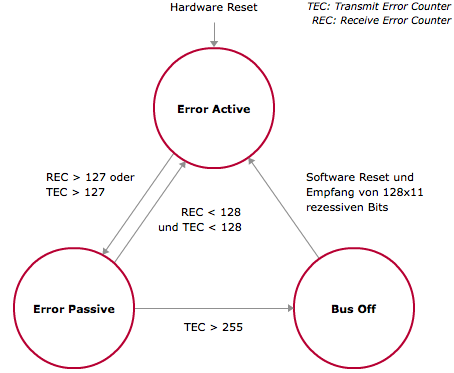
\includegraphics[width=0.9\textwidth]{figures/errcount}
\caption{Fehlerverfolgung \citep{VEC}} 
\label{pic:errcount}
\end{figure} 

\clearpage
\section{CAN Bus over Ethernet}
	
\subsection{Probleme}

Bei der Übertragung von CAN über Ethernet ergeben sich aufgrund der unterschiedlichen
Funktionsweisen beider Systeme grundlegende Probleme.

%TODO

\subsection{CAN Schnittstelle}

CAN Schnittstellen erlauben es, eine CAN-Bus Struktur an Ethernet Topologien anzubinden. 
Dies ermöglicht anderen Netzwerkgeräten mit den Teilnehmern im CAN-Bus und vice versa 
zu kommunizieren. Typischerweise wird eine CAN Schnittstelle verwendet, um den CAN Bus 
über Ethernet mit einem PC zu verbinden. Dies ermöglicht einen flexiblen Zugriff auf die 
CAN-Systeme über LAN oder sogar Internet. Die CAN Schnittstelle verhält sich dabei wie 
ein normaler CAN Knoten. \citep{STE}

Die CAN Nachrichten werden vom CAN Gateway in Ethernet Packete eingepackt und dann 
über die Ethernet Verbindung gesendet. Dabei gehen jedoch wichtige Eigenschaften des 
CAN-Busses verloren. Zum Beispiel wird das ACK-Feld im CAN-Frame nicht mehr vom 
eigentlichen Empfänger, dem PC, sondern direkt von der CAN Schnittstelle gesetzt. Dadurch 
kann nicht sichergestellt werden, ob die Nachricht auch tatsächlich fehlerfrei beim PC angekommen ist.
Abbildung \ref{gateway} zeigt die Topologie des Netzwerkes bestehend aus CAN-Netzwerk, 
CAN-Schnittstelle und Ethernet.

\begin{figure}[h] 
\centering
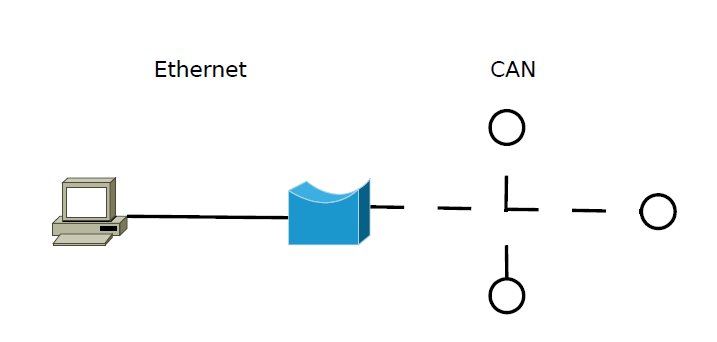
\includegraphics[width=0.7\textwidth]{figures/can_gateway}
\caption{CAN-Schnittstelle} 
\label{gateway}
\end{figure} 

\subsection{CAN Ethernet Bridge}

Die CAN Ethernet Bridge ermöglicht es, mehrere CAN Netzwerke miteinander über Ethernet 
(LAN oder Internet) zu verbinden. Abbildung \ref{bridge} zeigt zwei CAN Busse, die über 
Ethernet miteinander verbunden sind. Die CAN Bridges verhalten sich hierbei wieder wie 
CAN Teilnehmer. Auch hier gehen wichtige Eigenschaften des CAN-Busses, wie beispielsweise 
das Setzen des ACK-Feldes durch den Empfänger oder das eigentliche Zeitverhalten im 
jeweiligen CAN-Bus, verloren. Denn das ACK-Feld wird direkt von der Bridge und nicht von 
den eigentlichen Empfängern gesetzt.

Vorteil einer solchen Entkopplung der CAN Netzwerke ist, dass eine Filterung der gesendeten 
Nachrichten möglich ist, und somit der Datenfluss zwischen den CAN Netzwerken beeinflussbar 
ist. So können beispielsweise Fehler abgefangen und begrenzt werden. Ein weiterer Vorteil 
einer Entkopplung ist, dass das Zeitverhalten der Busse getrennt betrachtet werden kann 
und für Analysen anstatt eines riesigen Busses nur einen Teil des Busses betrachtet werden 
muss.

\begin{figure}[h] 
\centering
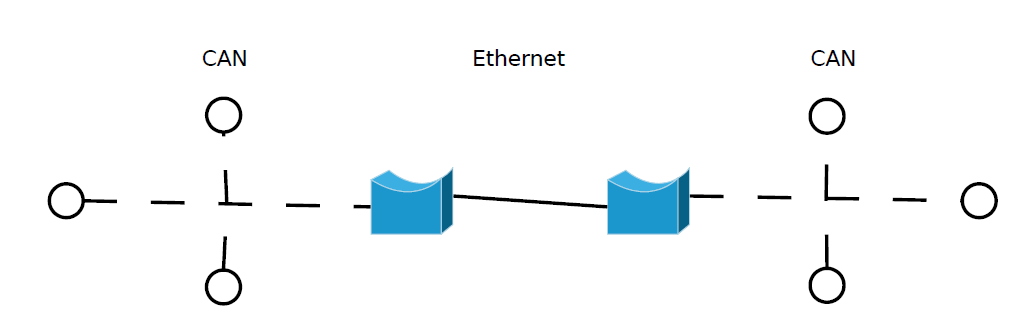
\includegraphics[width=0.8\textwidth]{figures/can_bridge}
\caption{CAN Ethernet Bridge} 
\label{bridge}
\end{figure}

\subsubsection{Transparente Bridge}

Wie bereits erwähnt, gehen bei dem bisher beschiebenen Bridge-System Eigenschaften
des CAN Bus verloren. Es stellt sich die Frage, ob es möglich ist einen CAN-Bus
streckenweise über Ethernet zu übertragen ohne dass Teilnehmer einen Unterschied zu
einem gewöhnlichen CAN-Bus erkennen können.

Um dies zu gewährleisten müssen alle Teilnehmer Nachrichten in der selben Reihenfolge
erhalten. Weiters müssen auftretende Fehler im gesamten System erkannt werden. Das
obige CAN Ethernet Bridge System erfüllt beide Anforderungen nicht, da die Bus
Arbitration separat für die beiden verbundenen Busse durchgeführt wird und das
ACK-Feld bereits von den Bridges gesetzt wird.

Letzteres verhindert, dass eine Station, die in ihrem CAN-Bus alleine ist, von
Übertragunsfehlern im anderen CAN-Bus erfährt.

Die separate Durchführung der Bus Arbitration kann dazu führen, dass zwei Frames, die
in unterschiedlichen CAN-Bussen zeitgleich gesendet werden, von Stationen im eigenen
Bus vor dem anderen Frame empfangen werden. Damit wäre die Reihenfolge, in der die
beiden Nachrichten empfangen werden dann in den beiden Bussen unterschiedlich.

Um die beiden Busse transparent zu verbinden, muss daher das Erscheinen einzelner
Bits in den Bussen so erfolgen, dass alle Stationen zur selben Zeit das gleiche Bit
sampeln können.

CAN sieht für unterschiedliche Bandbreiten verschiedene maximale Bus-Längen vor. Das
Propagation Delay bezeichnet jene Zeit, die ein gesendetes Bit benötigt, um an jedem
Punkt am Bus gelesen werden zu können. Um gleichzeitiges Lesen zu ermöglichen, muss
das System mit der transparenten Ethernet Bridge das Propagation Delay für die
maximale Bus-Länge bei der konfigurierten CAN-Bandbreite einhalten und alle Bits
einzeln über die Ethernet-Verbindung übertragen.

\paragraph{Beispiel}
Gegeben sind zwei CAN-Busse mit $20 kBit/s$ Bandbreite. Diese beiden Busse sollen
transparent über eine $100 m$ Fast Ethernet Leitung verbunden werden. Die maximale
Bus-Länge $l$ bei $20 kBit/s$ beträgt $2500 m$. Davon ausgehend, dass die
Ausbreitungsgeschwindigkeit in einem Kabel $v$ etwa $2/3$ der Lichtgeschwindigkeit beträgt,
ist das Propagation Delay $t_{pc} = \frac{l}{v_a}$ in einem $2500 m$ langen Bus etwa
$12,5 \mu s$.

Da in Ethernet nur Frames mit mindestens $64 Byte$ übertragen werden können, und ein
Frame vollständig gelesen werden muss, bevor man dessen Inhalt verwenden kann, muss
für die Übertragung eines Bits über die Ethernet-Leitung nicht nur das Propagation
Delay, sondern die gesamte Übertragungsdauer $t_t$ verwendet werden. Bei Fast
Ethernet auf einer $100 m$ Strecke beträgt diese $5,62 \mu s$. Sie wird berechnet aus
$\frac{Bits}{Bandbreite} + Propagation Delay$.

Damit ergibt sich für das Propagation Delay des gesamten Systems $t_{pe} = t_{p_1} +
t_{p_2} + t_t$, wobei $t_{p_1}$ und $t_{p_2}$ die Propagation Delays der beiden
CAN-Busse sind. Um die oben genannten Anforderungen zu erfüllen, muss gelten $t_{pe}
\leq t_{pc}$. Das maximale Propagation Delay der beiden CAN-Busse darf daher
höchstens $t_{pc} - t_t = 6,88 \mu s$ betragen. Die maximal mögliche Gesamtlänge der
beiden Busse schrumpft damit auf $1376 m$.

Somit ergibt sich für das gesamte System eine maximale Länge von $1476 m$. Dies liegt
deutlich unter den $2500 m$, die mit einem gewöhnlichen CAN-Bus möglich gewesen
wären. Da die Ausbreitungsgeschwindigkeit für Ethernet und CAN gleich ist, ist es
nicht möglich durch die Verwendung einer transparenten Ethernet Bridge eine längere
Strecke abzudecken als mit CAN alleine.

Obiges Beispiel geht von einigen vereinfachenden Annahmen aus:
\begin{itemize}
        \item Die Übertragung über die Ethernet-Leitung funktioniert immer
                fehlerfrei.
        \item Die Ethernet-Strecke hat nur zwei Teilnehmer (die beiden Bridges) und
                wird im Full-Duplex Modus betrieben.
        \item Die Bridges und sämtliche Netzwerkgeräte zwischen ihnen (z.B. Repeater)
                verursachen keine Verzögerung.
\end{itemize}

Wie bereits erwähnt, lässt sich durch die transparente Ethernet Bridge kein Gewinn
erzielen, da weder die maximale Länge, noch die Bandbreite des Systems erhöht werden
kann.

Allerdings ist es durch den hohen Overhead der Ethernet-Übertragung (ein Frame pro
Bit) eventuell möglich mehrere synchronisierte CAN-Busse über die gleiche
Ethernet-Leitung zu übertragen und so zu bündeln, um Kabel einzusparen.

\subsection{Implementierungen}

%TODO

\newpage \addcontentsline{toc}{section}{Abbildungen} \listoffigures

\newpage \addcontentsline{toc}{section}{Literatur}
%\bibliographystyle{abbrv} 
\bibliographystyle{alphadin}
\bibliography{quellen}
